\documentclass[border=2pt]{standalone}
\usepackage{pgfplots}
\pgfplotsset{compat=1.18}
\definecolor{red}{rgb}{0.7,0.11,0.11}
\definecolor{blue}{rgb}{0.0,0.20,0.42}
\definecolor{green}{rgb}{0.11,0.35,0.02}
\begin{document}
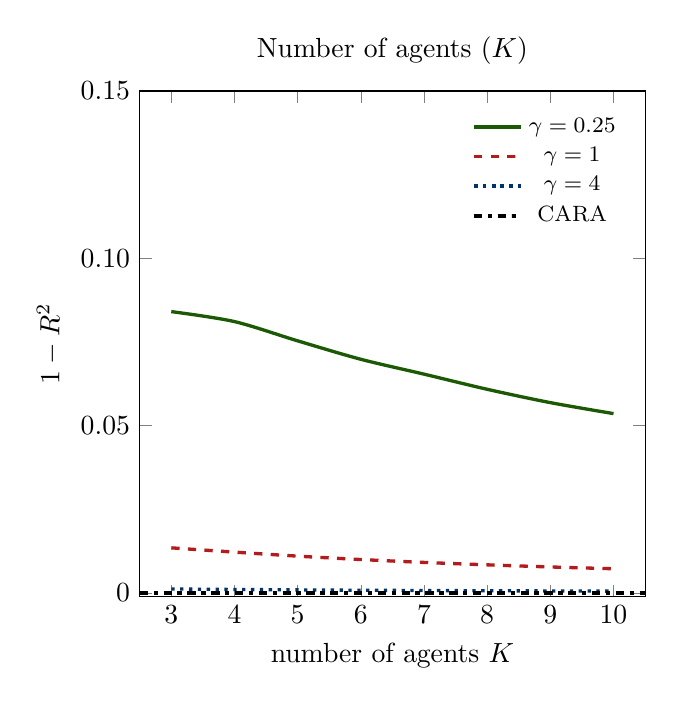
\begin{tikzpicture}
\begin{axis}[
    width=8cm, height=8cm,
    xmin=2.5, xmax=10.5,
    ymin=-0.001, ymax=0.15,
    xtick={3,4,5,6,7,8,9,10},
    ytick={0,0.05,0.1,0.15},
    yticklabels={0,0.05,0.10,0.15},
    xlabel={number of agents $K$},
    ylabel={$1 - R^2$},
    title={Number of agents ($K$)},
    legend pos=north east,
    legend style={fill=none, draw=none, font=\footnotesize},
    smooth,
]
\addplot[very thick, color=green, smooth] coordinates {(3,0.0840731) (4,0.0810895) (5,0.0753357) (6,0.0698296) (7,0.0653901) (8,0.0608647) (9,0.0568783) (10,0.0535977)};
\addplot[very thick, color=red, dashed, smooth] coordinates {(3,0.0134878) (4,0.0122128) (5,0.0110119) (6,0.01) (7,0.00913557) (8,0.00841322) (9,0.007778) (10,0.00724019)};
\addplot[very thick, color=blue, dotted, smooth] coordinates {(3,0.00119451) (4,0.00105344) (5,0.000928624) (6,0.00082586) (7,0.000739966) (8,0.000670909) (9,0.000610704) (10,0.000561077)};
\addplot[ultra thick, color=black, dashdotted]
    coordinates {(2.5,0)(10.5,0)};
\addlegendentry{$\gamma = 0.25$}
\addlegendentry{$\gamma = 1$}
\addlegendentry{$\gamma = 4$}
\addlegendentry{CARA}
\end{axis}
\end{tikzpicture}
\end{document}
